% AIAA student-conference paper 1 of 2: the impossibility result (11-page limit).
% Companion: ../algorithm/main.tex. Shared format: ../aiaa-format.tex.
% Build: latexmk -pdf main.tex   (from this directory)
% Shared format for the two AIAA student-conference papers in this folder (impossibility/ and algorithm/).
% AIAA Meeting Paper (conference) format, reproduced from the published instructions
% ("Preparation of Papers for AIAA Technical Conferences"): letter paper, 1 in margins, Times 10 pt, single column,
% single spaced; title bold 24 pt; abstract bold, indented 0.5 in each side; section headings bold 11 pt, centered,
% Roman numerals; subsections bold flush left with capital letters; sub-subsections italic with arabic numerals;
% captions bold ("Fig. 1" below figures, "Table 1" above tables); footnote symbols; numbered references.
% To use AIAA's own class instead, replace everything between the two "FORMAT" markers by
%     \documentclass[conf]{new-aiaa}  plus the packages and macros marked KEEP,
% and move the title, authors and abstract into that class's \title, \author, \affil and abstract commands.
% ----------------------------------------------------------------------------------------------- FORMAT (begin)
\documentclass[10pt,letterpaper]{article}
\usepackage[margin=1in]{geometry}
\usepackage[T1]{fontenc}
\usepackage{amsmath,amsthm}            % KEEP
\usepackage{txfonts}                   % Times text and math
\usepackage{graphicx,booktabs,array}   % KEEP
\usepackage{enumitem}                  % KEEP
\usepackage{titlesec}
\usepackage[labelfont=bf,textfont=bf,labelsep=quad,justification=centering,skip=6pt]{caption}
\usepackage{lettrine}
\usepackage[numbers,sort&compress]{natbib}
\usepackage[hidelinks]{hyperref}
\urlstyle{same}
\renewcommand{\figurename}{Fig.}
\captionsetup[table]{position=above}
\titleformat{\section}{\normalfont\fontsize{11}{13}\selectfont\bfseries\centering}{\Roman{section}.}{0.5em}{}
\titleformat{\subsection}{\normalfont\normalsize\bfseries}{\Alph{subsection}.}{0.5em}{}
\titleformat{\subsubsection}{\normalfont\normalsize\itshape}{\arabic{subsubsection}.}{0.5em}{}
\titlespacing*{\section}{0pt}{12pt plus 2pt minus 2pt}{6pt}
\titlespacing*{\subsection}{0pt}{9pt plus 2pt minus 1pt}{3pt}
\titlespacing*{\subsubsection}{0pt}{6pt plus 1pt minus 1pt}{2pt}
\renewcommand{\thefootnote}{\fnsymbol{footnote}}
\setlength{\parindent}{0.2in}
\setlength{\parskip}{0pt}
\setlength{\bibsep}{2.5pt}
\renewcommand{\bibfont}{\small}
\makeatletter
\renewcommand{\@biblabel}[1]{[#1]}
\makeatother
\newenvironment{aiaaabstract}{\begin{list}{}{\setlength{\leftmargin}{0.5in}\setlength{\rightmargin}{0.5in}%
  \setlength{\listparindent}{0.2in}\setlength{\itemindent}{0.2in}\setlength{\topsep}{10pt}}\item\bfseries}{\end{list}}
% ------------------------------------------------------------------------------------------------- FORMAT (end)
% KEEP: theorem environments and notation
\newtheoremstyle{aiaa}{4pt}{4pt}{\itshape}{}{\bfseries}{.}{0.5em}{}
\theoremstyle{aiaa}
\newtheorem{theorem}{Theorem}
\newtheorem{lemma}{Lemma}
\newtheorem{proposition}{Proposition}
\newcommand{\norm}[1]{\lVert #1\rVert}
\newcommand{\ip}[2]{\langle #1,#2\rangle}
\newcommand{\ez}{e_z}
\newtheorem{corollary}{Corollary}

\newtheorem{definition}{Definition}
\newcommand{\R}{\mathbb{R}}
\newcommand{\F}{F_{t_f}}
\newcommand{\FX}{F^{X}_{t_f}}
\newcommand{\us}{\_\allowbreak}
\newcommand{\lean}[1]{\texttt{\small #1}}

\begin{document}
\begin{center}
{\fontsize{24}{28}\selectfont\bfseries Lossless Convexification Is Impossible for Attitude-Rate-Limited Powered Descent\par}
\vspace{14pt}
% Authors: Regional Student Conference rules require every author to be identified in the first-page footnote by
% status (Undergraduate / Master's / Doctoral Student or Faculty Member), role (Contributing Student Author or Mentor
% Author) and AIAA membership. Undergraduate and Graduate categories allow at most two Contributing Student Authors;
% the Team category needs three or more. Contributing Student Authors are listed before Mentor Authors.
% A student may be a Contributing Student Author on only ONE paper in the High School, Undergraduate or Graduate
% category, but on more than one paper in the Team category. See ../README.md before choosing authors for the two papers.
{\large [First A. Author]\footnote{[Undergraduate] Student, [Daniel Guggenheim School of Aerospace Engineering], AIAA University Student
Member and Contributing Student Author.} and [Second B. Author]\footnote{[Undergraduate] Student, [Daniel Guggenheim School of
Aerospace Engineering], AIAA University Student Member and Contributing Student Author.}\par}
{\large\itshape Georgia Institute of Technology, Atlanta, Georgia, 30332\par}
\vspace{10pt}
{\large [Faculty C. Mentor]\footnote{[Professor], [Daniel Guggenheim School of Aerospace Engineering], [AIAA member grade], Mentor Author.}\par}
{\large\itshape Georgia Institute of Technology, Atlanta, Georgia, 30332\par}
\end{center}

\begin{aiaaabstract}
Lossless convexification solves three-degree-of-freedom powered-descent guidance exactly as one convex program. We prove that
no formulation of that kind exists once the thrust direction is tied to a body that turns at a finite rate. A convex program
that receives the initial position and velocity through affine constraints, and that is feasible exactly when a landing
exists, forces the set of initial states from which a landing exists to be convex. For a vehicle with a rate-limited body
axis, a gimbal cone, and a positive minimum throttle, under altitude and glide-slope constraints, we show that this set is not
convex for any final time: a maneuver that dives to one side and then brakes can land, and so can its mirror image, but no
maneuver lands from the average of their initial states. The proof uses only the triangle inequality on the sphere. It
extends to depleting mass, upright touchdown, six-degree-of-freedom attitude kinematics, and free final time on bounded
windows, and these statements are checked by the Lean~4 proof assistant. We also bound the size of the effect, which is small
for descents that begin in the air, and report what is proved and what is only observed numerically when the gimbal is the
sole source of torque. The result excludes exactness and nothing else: a convex program that returns only flyable
trajectories remains possible, and we outline one.
\end{aiaaabstract}

\section{Nomenclature}
{\renewcommand{\arraystretch}{1.0}\noindent
\begin{tabular}{@{}l@{\ \,=\ \,}l@{\hspace{0.2in}}l@{\ \,=\ \,}l@{}}
$a$ & thrust per unit mass, $T/m$, m/s$^2$ & $t_f$ & final time, s \\
$a_{\max}$ & upper bound on $a$, m/s$^2$ & $u$ & horizontal unit vector \\
$A_b$ & $\rho_2/m_0-g_0$, m/s$^2$ & $W$ & weighted thrust integral, m \\
$b$ & unit vector along the body axis & $X$ & set of admissible states \\
$C$ & feasible set of a convex program & $\alpha$ & mass flow per unit thrust, kg/(N\,s) \\
$d$ & unit vector along the thrust & $\gamma_{gs}$ & glide-slope angle, rad \\
$\ez$ & unit vector pointing up & $\delta$ & gimbal-angle limit, rad \\
$\F$, $\FX$ & sets of initial data with a landing & $\theta$ & initial data $(r_0,v_0)$ \\
$g_0$ & gravitational acceleration, m/s$^2$ & $\theta^*$, $\theta_m$ & witness data and midpoint data \\
$m$, $m_0$ & mass and initial mass, kg & $\Lambda$ & $r_0+s^*v_0$, m \\
$r$, $v$ & position and velocity, m and m/s & $\rho_1$, $\rho_2$ & thrust limits, N \\
$R_\pi$ & rotation by $\pi$ about the vertical & $\omega$ & limit on the turn rate of the body axis, rad/s \\
$s^*$ & switch time from dive to brake, s & $(\cdot)_h$, $(\cdot)_z$ & horizontal and vertical parts \\
\end{tabular}}

\section{Introduction}
\lettrine{L}{ossless} convexification (LCvx) is the reason powered-descent guidance can be solved on board. The thrust
magnitude of a rocket engine is bounded below as well as above, so the admissible thrust set is an annulus and the guidance
problem is not convex. LCvx replaces the annulus by a convex cone in a lifted space and proves that an optimal solution of
the relaxed second-order cone program satisfies the original constraints
\cite{acikmese2007,blackmore2010,acikmese2011,acikmese2013}. One convex program is solved, no initial guess is needed, and
the answer is exact. The result has been extended to pointing constraints and to classes of state constraints
\cite{acikmese2013,harris2014}, and it has flown \cite{malyuta2022}.

Every one of these results treats the thrust direction as a control that may change instantly. A real lander points its
thrust by pointing its body, and the body turns at a finite rate. When the attitude is included, guidance is done by
successive convexification, which linearizes the dynamics about a trial trajectory and iterates
\cite{mao2016,szmuk2018,szmuk2020}. That raises a natural question, which to our knowledge has not been answered: is the
iteration necessary, or is there a lossless convexification of the attitude-coupled problem that has not been found yet?

This paper answers the question for the class of programs to which LCvx belongs. The contributions are as follows.

1) An obstruction (Sec.~\ref{sec:obstruction}). If a convex program takes the initial position and velocity through affine
constraints and is feasible exactly at the initial data from which a landing exists, then the set of such data is convex.
The statement is elementary; its use is that it turns a question about all possible reformulations into a question about one
set.

2) A proof that the set is not convex (Sec.~\ref{sec:dive}). For a body axis that turns at a rate of at most $\omega$, a
gimbal cone, and a positive minimum throttle, with altitude and glide-slope constraints, the set of landable initial data is
not convex for any final time. The simplest witnesses of nonconvexity hold minimum throttle throughout, and for a vehicle
that cannot hover at minimum throttle they start below the ground; the dive-then-brake maneuver used here does not.

3) Machine-checked proofs (Sec.~\ref{sec:lean}). The obstruction, the nonconvexity theorem, and its extensions to depleting
mass, upright touchdown, six-degree-of-freedom (6-DOF) attitude kinematics, and free final time are formalized in Lean~4
\cite{lean4,mathlib}.

4) An account of how much the result matters (Secs.~\ref{sec:size} and \ref{sec:tvc}). We give an explicit lower bound on the
distance from the set to a point of its convex hull, show that it is small for an 80-kg lander descending from the air,
and separate what is proved from what is observed numerically for a vehicle whose only torque comes from its gimbal.

The result is about exactness. It does not say that attitude-coupled guidance must be iterative, and Sec.~\ref{sec:possible}
explains what remains possible, including a single convex program for a gimbaled lander that returns only flyable
trajectories and gives up a small set of feasible landings, which is the best outcome the present result allows. The Lean
sources, the certificates, and the software behind every number in this paper are public \cite{repo}.

\section{Problem Statement}\label{sec:problem}
\subsection{Vehicle Model}
The translational dynamics are those of the LCvx literature,
\begin{equation}\label{eq:dyn}
\dot r=v,\qquad \dot v=a\,d-g_0\ez,\qquad \dot m=-\alpha T,\qquad a=T/m ,
\end{equation}
with thrust magnitude $T(t)\in[\rho_1,\rho_2]$, $\rho_1>0$, thrust direction $d(t)$ a unit vector, and $\alpha\ge0$. The
initial mass $m_0$ satisfies $m_0-\alpha\rho_2t_f>0$, so that $a\le a_{\max}=\rho_2/(m_0-\alpha\rho_2t_f)$. The attitude enters
through the unit body axis $b(t)$, which starts vertical, $b(0)=\ez$, and turns at a rate of at most $\omega$,
$0<\omega<\infty$:
\begin{equation}\label{eq:AL}
\ip{b(s)}{b(s')}\ \ge\ \cos\bigl(\omega\lvert s-s'\rvert\bigr)\qquad\text{whenever }\omega\lvert s-s'\rvert\le\pi .
\end{equation}
Inequality~\eqref{eq:AL} holds if and only if $b$ is absolutely continuous with $\dot b=\Omega\times b$ and the part of
$\Omega$ perpendicular to $b$ is bounded by $\omega$; the roll rate is unrestricted. The thrust is held within a gimbal cone
about the body axis,
\begin{equation}\label{eq:gimbal}
\ip{d(t)}{b(t)}\ \ge\ \cos\delta,\qquad 0<\delta<\pi/2 ,
\end{equation}
and the gimbal is fast, so $d$ is any measurable function that satisfies Eq.~\eqref{eq:gimbal}. A control is a triple
$c=(T,b,d)$ with these properties. Roll does not move the thrust axis of an axisymmetric vehicle, so this model has five
degrees of freedom (5-DOF): three of translation and two of pointing.

The model is deliberately the mildest one in which attitude matters. It has no rotational inertia and no coupling between
the gimbal and the rotation of the body; it adds to the 3-DOF problem only the requirement that the thrust direction stay
near an axis that cannot jump. Section~\ref{sec:tvc} returns to the vehicle whose body is turned by the gimbal itself.

\subsection{Landing Sets}
The initial data are $\theta=(r_0,v_0)\in\R^6$. The final time $t_f$, the initial mass, and the initial attitude are fixed,
and landing means $r(t_f)=0$ and $v(t_f)=0$. The state must remain in
\begin{equation}\label{eq:X}
X=\bigl\{(r,v):\ r_z\ge0,\ \ r_z\ge\tan\gamma_{gs}\,\norm{r_h}\bigr\},\qquad 0\le\gamma_{gs}<\pi/2 ,
\end{equation}
that is, above the ground and inside a glide-slope cone; $\gamma_{gs}=0$ leaves the altitude constraint alone.

\begin{definition}
$\F$ is the set of data $\theta$ from which some control lands at $t_f$. $\FX\subseteq\F$ is the set of data from which
some control lands with $(r(t),v(t))\in X$ for all $t$.
\end{definition}

\subsection{Convex Programs and Losslessness}
\begin{definition}\label{def:program}
A uniform convex relaxation is a convex set $C\subseteq\R^6\times Y$, where $Y$ is any real vector space. Its slice
$C_\theta=\{y:(\theta,y)\in C\}$ is the feasible set of the program at the data $\theta$. The relaxation is lossless for a
set $F\subseteq\R^6$ if $C_\theta$ is nonempty exactly when $\theta\in F$.
\end{definition}
The space $Y$ holds everything except the data: states, relaxed controls, slack variables, a discretization, or functions of
time. The definition asks for two properties at once. The program is \emph{sound} if it is feasible only at data from which
a landing exists, and \emph{complete} if it is feasible at all such data. LCvx has both.

Three remarks fix the scope. First, the class contains LCvx. Every LCvx formulation we know imposes the initial condition as
a linear equality $x(0)=x_0$ on top of a convex constraint set in the remaining variables, so its feasible set is convex
jointly in the data and the variables; the change of variables to the logarithm of the mass \cite{acikmese2007} acts on
$Y$ only. Second, the usual definition of losslessness refers to optimal solutions: whenever the relaxed problem is feasible,
its optimum is attained at a point that satisfies the original constraints. That definition implies the one above, because an
attained relaxed optimum certifies a landing. The results below therefore hold for every cost. Third, the class is
restricted on purpose. If the data may enter a program in an arbitrary nonlinear way, any set is the preimage of a convex
one and the question has no content; programs over occupation measures \cite{lasserre2008}, in which the initial state
enters as a point mass, are convex and can be exact, but they are infinite-dimensional and are set up for one instance at a
time. They are outside the class, and outside what LCvx means in guidance practice.

\section{The Obstruction}\label{sec:obstruction}
\begin{theorem}\label{thm:A}
If a uniform convex relaxation $C$ is lossless for $F$, then $F$ is the projection of $C$ onto the data, and $F$ is convex.
Consequently, if $F$ is not convex, no uniform convex relaxation is lossless for $F$, for any cost.
\end{theorem}
\begin{proof}
$\theta$ belongs to the projection of $C$ if and only if $C_\theta$ is nonempty, which by losslessness holds if and only if
$\theta\in F$. The projection is a linear image of a convex set and is therefore convex.
\end{proof}

The theorem also says how an attempted relaxation fails. Suppose $C$ is complete, as any relaxation that merely enlarges
the constraint set is. Then the projection of $C$ is a convex set that contains $F$, hence contains the convex hull of $F$,
and the program reports a landing at every point of the hull that is not in $F$. If such a point lies at distance $\Gamma$
from $F$, no complete program detects infeasibility to better than $\Gamma$.

Theorem~\ref{thm:A} is consistent with 3-DOF LCvx. When the thrust direction is free, the set of velocity and position
increments that the thrust can produce is the integral of a set-valued function, which is convex by Aumann's theorem
\cite{aumann1965} whatever the pointwise thrust set is, and $\F$ is convex. The theorem identifies what a positive result
needs and what a negative result must show. The rest of the paper shows that $\FX$ is not convex.

\section{The Landing Set Is Not Convex}\label{sec:dive}
\subsection{An Identity and Two Lemmas}
Fix a switch time $s^*\in(0,t_f)$. Integrating Eq.~\eqref{eq:dyn} twice and imposing $r(t_f)=v(t_f)=0$ gives, for every
control that lands from $\theta$,
\begin{equation}\label{eq:lambda}
\Lambda(\theta):=r_0+s^*v_0=W(c)+\kappa\,\ez,\qquad W(c)=\int_0^{t_f}(s-s^*)\,a\,d\;\mathrm ds,\qquad
\kappa=g_0t_f\Bigl(s^*-\frac{t_f}{2}\Bigr).
\end{equation}
The weight $s-s^*$ is negative before $s^*$ and positive after it. The vertical component $\Lambda_z$ is a linear function
of the data that is unchanged by rotation about the vertical, and making it large asks for as little upward thrust as
possible before $s^*$ and as much as possible after. That is a dive followed by a brake.

\begin{lemma}[Triangle inequality on the sphere]\label{lem:tri}
Let $x,y,z$ be unit vectors and $\alpha,\beta\ge0$ with $\alpha+\beta\le\pi$, $\ip xy\ge\cos\alpha$, and
$\ip yz\ge\cos\beta$. Then $\ip xz\ge\cos(\alpha+\beta)$. If equality holds, $\alpha+\beta<\pi$, and $0<\beta<\pi$, then
$\ip yz=\cos\beta$ and $x=\cos\alpha\,y-(\sin\alpha/\sin\beta)(z-\cos\beta\,y)$.
\end{lemma}
\begin{proof}
Write $\ip xy=\cos p$ and $\ip yz=\cos q$ with $0\le p\le\alpha$ and $0\le q\le\beta$, and let $x'=x-\cos p\,y$ and
$z'=z-\cos q\,y$, which are perpendicular to $y$ and have norms $\sin p$ and $\sin q$. Then
$\ip xz=\cos p\cos q+\ip{x'}{z'}\ge\cos p\cos q-\sin p\sin q=\cos(p+q)\ge\cos(\alpha+\beta)$. Equality requires $p=\alpha$
and $q=\beta$, because the cosine is strictly decreasing on $[0,\pi]$, and $x'=-(\sin\alpha/\sin\beta)z'$.
\end{proof}

With $x=d$, $y=b$, and $z=\ez$, the lemma reads as follows. If the body is tilted by at most $\varphi$ from the vertical
and $\delta+\varphi<\pi$, then $d_z\ge\cos(\delta+\varphi)$. If equality holds and $\varphi>0$, the body is tilted by exactly
$\varphi$, toward some horizontal unit vector $u$, and the thrust is deflected the full gimbal angle further in the same
direction:
\begin{equation}\label{eq:extremal}
b=\cos\varphi\,\ez+\sin\varphi\,u,\qquad d=\cos(\delta+\varphi)\,\ez+\sin(\delta+\varphi)\,u .
\end{equation}

\begin{lemma}[Rigidity]\label{lem:rigid}
Let $b(s)=\cos\psi\,\ez+\sin\psi\,u$ and $b(s')=\cos\psi'\,\ez+\sin\psi'\,u'$ with $\psi,\psi'\in(0,\pi)$ and $u,u'$
horizontal unit vectors. If $\ip{b(s)}{b(s')}\ge\cos(\psi-\psi')$, then $u=u'$.
\end{lemma}
\begin{proof}
$\ip{b(s)}{b(s')}-\cos(\psi-\psi')=\sin\psi\sin\psi'\,(\ip u{u'}-1)$, which is nonnegative only if $\ip u{u'}=1$.
\end{proof}
Lemma~\ref{lem:rigid} is where the finite rate acts. A body that tilts as fast as the rate limit allows has no rate left
to change the direction in which it tilts.

\subsection{Main Theorem}
\begin{theorem}\label{thm:Bstar}
Consider the model of Sec.~\ref{sec:problem} with $\rho_1>0$, $0<\omega<\infty$, $0<\delta<\pi/2$, $\alpha\ge0$, and
$A_b=\rho_2/m_0-g_0>0$. Let $s^*\in(0,t_f)$ satisfy
\begin{equation}\label{eq:S}
\text{(S1)}\ \ \omega s^*\le\min\Bigl(\delta,\frac\pi2-\delta\Bigr),\qquad
\text{(S2)}\ \ g_0s^*<A_b(t_f-s^*),\qquad
\text{(S3)}\ \ \tan\gamma_{gs}\,a_{\max}s^{*2}\le A_b(t_f-s^*)^2 .
\end{equation}
Then there are data $\theta^*\in\FX$ such that $R_\pi\theta^*\in\FX$ and the midpoint
$\theta_m=\tfrac12(\theta^*+R_\pi\theta^*)$ is not in $\F$. Conditions (S1) to (S3) hold for every sufficiently small $s^*$,
so $\FX$ is not convex for any $t_f>0$.
\end{theorem}
\begin{proof}
Write $a_T$ for the thrust acceleration produced by a throttle history $T$.

\emph{Step 1 (bound for a fixed throttle).} Let $c=(T,b,d)$ be any control. By Eq.~\eqref{eq:AL} with $s'=0$, the tilt of $b(s)$
is at most $\omega s$. On $[0,s^*]$, $\delta+\omega s\le\pi/2$ by (S1), so Lemma~\ref{lem:tri} gives
$d_z\ge\cos(\delta+\omega s)\ge0$. On $(s^*,t_f]$, $d_z\le1$. Because the weight in Eq.~\eqref{eq:lambda} is negative before
$s^*$ and positive after,
\begin{equation}\label{eq:V}
W_z(c)\ \le\ V(T):=-\int_0^{s^*}(s^*-s)\,a_T\cos(\delta+\omega s)\,\mathrm ds+\int_{s^*}^{t_f}(s-s^*)\,a_T\,\mathrm ds .
\end{equation}

\emph{Step 2 (the bound is attained).} Fix a horizontal unit vector $u$. The dive-then-brake control $c^T_u$ uses, on
$[0,s^*]$, the body axis and thrust direction of Eq.~\eqref{eq:extremal} with $\varphi=\omega s$; after $s^*$ it holds the
body at its tilt $\omega s^*$ and points the thrust straight up, $d=\ez$. It is admissible: the body turns at the rate
$\omega$ and then stops, the gimbal angle is $\delta$ during the dive, and during the brake it is $\omega s^*\le\delta$ by (S1).
It attains equality in Eq.~\eqref{eq:V}.

\emph{Step 3 (full throttle on the brake).} Replacing $T$ by $\rho_2$ on $(s^*,t_f]$ leaves $a_T$ unchanged before $s^*$
and does not decrease it afterward, because for $s>s^*$ the mass is then smallest and the thrust largest. Hence $V$ does not
decrease, and it increases unless $T=\rho_2$ almost everywhere on $(s^*,t_f]$.

\emph{Step 4 (best throttle).} $V^*=\sup_TV(T)$ is attained at some $T^*$. For $\alpha=0$ the maximizer is explicit:
$\cos(\delta+\omega s)\ge0$ on the dive by (S1), so $T^*=\rho_1$ before $s^*$ and $\rho_2$ after. For $\alpha>0$, $V$ is
continuous in the weak-$*$ topology on the compact set of throttle histories, and a maximizer exists.

\emph{Step 5 (the witnesses satisfy the state constraints).} Let $\theta^*$ be the data from which $c^{T^*}_u$ lands. On
the brake $d=\ez$, so the trajectory is vertical there and $\dot v_z\ge A_b$; hence $v_z(t)\le-A_b(t_f-t)$ and
$r_z(t)\ge\tfrac12A_b(t_f-t)^2$. On the dive $d_z\ge0$, so $\dot v_z\ge-g_0$ and
$v_z(t)\le-A_b(t_f-s^*)+g_0s^*<0$ by (S2). The altitude therefore decreases monotonically to zero and is positive before
$t_f$. The lateral speed is at most $a_{\max}(s^*-t)$ on the dive, so $\norm{r_h}\le\tfrac12a_{\max}s^{*2}$, whereas
$r_z\ge\tfrac12A_b(t_f-s^*)^2$ there, and (S3) gives the glide slope. Thus $\theta^*\in\FX$. The model is invariant under
rotation about the vertical, so $c^{T^*}_{-u}$ lands from $R_\pi\theta^*$ and $R_\pi\theta^*\in\FX$.

\emph{Step 6 (the midpoint is not landable).} The midpoint $\theta_m$ has the vertical components of $\theta^*$ and zero
horizontal components, so $\Lambda(\theta_m)=(V^*+\kappa)\,\ez$. Suppose a control $c=(T,b,d)$ lands from $\theta_m$. By
Eq.~\eqref{eq:lambda}, $W(c)=V^*\ez$, so $V^*=W_z(c)\le V(T)\le V^*$ and every inequality used in Step~1 is an equality
almost everywhere. On the dive this means $d_z=\cos(\delta+\omega s)$, and Eq.~\eqref{eq:extremal} gives, for almost every
$s\in(0,s^*]$, a horizontal unit vector $u(s)$ with $b(s)=\cos\omega s\,\ez+\sin\omega s\,u(s)$ and
$d(s)=\cos(\delta+\omega s)\,\ez+\sin(\delta+\omega s)\,u(s)$. For two such times $s<s'$, Eq.~\eqref{eq:AL} gives
$\ip{b(s)}{b(s')}\ge\cos(\omega s'-\omega s)$, and Lemma~\ref{lem:rigid} gives $u(s)=u(s')$. So $u(s)$ is a constant $u_0$.
On the brake, equality means $d_z=1$, that is, $d=\ez$. The horizontal part of $W(c)$ is then
\begin{equation}
W_h(c)=-\Bigl(\int_0^{s^*}(s^*-s)\,a_T\sin(\delta+\omega s)\,\mathrm ds\Bigr)u_0\ \ne\ 0 ,
\end{equation}
because $a_T>0$ and $0<\delta+\omega s\le\pi/2$. This contradicts $W_h(c)=\Lambda_h(\theta_m)=0$.
\end{proof}

\begin{corollary}\label{cor:main}
Under the hypotheses of Theorem~\ref{thm:Bstar}, for every final time $t_f>0$, no uniform convex relaxation is lossless for
the powered-descent problem with a rate-limited body axis, a gimbal cone, and altitude and glide-slope constraints.
\end{corollary}

Figure~\ref{fig:witness} shows the two witnesses for constants close to those of an 80-kg lander. The mechanism is visible
in Step~6. Among all controls, the witnesses make $\Lambda_z$ as large as it can be, and any control that matches them must
tilt at the full rate from the first instant, which fixes a direction; a control cannot do that and have no net lateral
effect. With an unlimited rate the body can alternate between the two directions arbitrarily fast and the midpoint becomes
landable, which is the 3-DOF situation. With zero rate the attitude is fixed and the thrust direction can alternate on the
gimbal cone instead. A finite, positive rate limit is what the obstruction needs. The altitude constraint is not what
causes it, since $\theta_m$ fails to be landable even without state constraints; the brake phase exists so that the witnesses
satisfy the constraints.

\begin{figure}[t]\centering
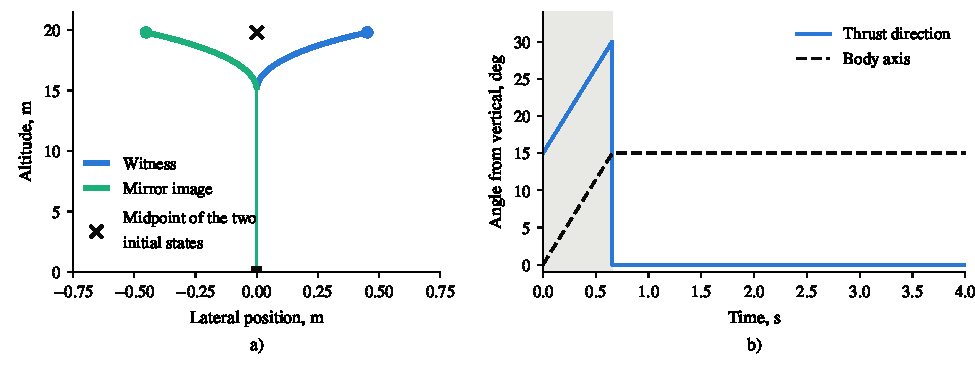
\includegraphics[width=6.5in]{figures/witness.pdf}
\caption{Witnesses of Theorem~\ref{thm:Bstar} for $\rho_1/m_0=5$~m/s$^2$, $\rho_2/m_0=12.5$~m/s$^2$, $\delta=15$~deg,
$\omega=0.4$~rad/s, $s^*=\delta/\omega$, $t_f=4$~s, and constant mass: a)~the two trajectories, with the dive drawn thick and
the lateral scale enlarged; b)~the attitude and thrust direction, with the dive shaded.}\label{fig:witness}
\end{figure}

\subsection{Extensions}\label{sec:ext}
The same proof covers the following cases; the changes are indicated.

\emph{Upright touchdown.} If $t_f\ge2s^*$, the witness can return its body axis to the vertical on $[s^*,2s^*]$ at the rate
$\omega$. The gimbal angle needed to keep $d=\ez$ stays below $\delta$, and nothing else changes. The theorem therefore
holds with the terminal condition $b(t_f)=\ez$.

\emph{Six degrees of freedom.} Let the attitude be a rotation matrix whose angular velocity is bounded by $\omega$, with any
roll motion. Its third column satisfies Eq.~\eqref{eq:AL}, so every 6-DOF control projects to a control of the present
model, and the witnesses lift to rotations about a fixed horizontal axis with zero roll. The 6-DOF landing set is contained
in $\F$ and contains the witnesses, so the theorem holds verbatim.

\emph{Free final time.} For a window $[t_a,t_b]$ with $s^*<t_a$ and (S1) to (S3) at $t_a$ with $a_{\max}$ evaluated at
$t_b$, the union of the sets $\FX$ over $t_f\in[t_a,t_b]$ is not convex. The maximum of $\Lambda_z$ over the union is
attained by the witnesses of some final time in the window. If the union were convex, their midpoint would be landable at
some final time $t'$ in the window and would attain the maximum of $\Lambda_z$ there, and Step~6 at $t'$ gives the
contradiction. A search over the final time with a convex program at each value is therefore not lossless either.

\emph{Other constraints.} Any additional closed constraint that is invariant under $R_\pi$ and satisfied by the witnesses can
be added, for example a tilt limit of at least $\omega s^*$.

\section{Machine-Checked Proofs}\label{sec:lean}
The obstruction is short, but it is easy to misstate: how the data enter, the terminal attitude, the state constraints, and
the sign conventions all matter. Its core was therefore formalized in Lean~4 with the Mathlib library
\cite{lean4,mathlib}. Table~\ref{tab:lean} lists the main statements. The project contains no unproved step, and each of
the 126 declarations audited by its verification script depends only on the three standard axioms of classical Lean
mathematics. The formal
statement of Theorem~\ref{thm:Bstar} assumes constant bounds $0<a_{\min}\le a\le a_{\max}$ on the thrust acceleration, or
explicit mass depletion with $0<\rho_1<\rho_2$ and $\alpha>0$; it assumes $\omega s^*\le\delta$ and
$\delta+\omega s^*\le\pi/2$, which together are (S1); and it replaces (S2) and (S3) by the single condition
$(a_{\max}+2\tan\gamma_{gs}\,a_{\min})s^{*2}\le(a_{\max}-g_0)(t_f-s^*)^2$. A separate lemma shows that such an $s^*$ exists
for every $t_f$. With mass depletion the maximizing throttle of Step~4 is constructed explicitly, so the formal proof does
not use weak-$*$ compactness.

\begin{table}[t]\centering
\caption{Statements checked in Lean 4}\label{tab:lean}
\small
\begin{tabular}{@{}>{\raggedright\arraybackslash}p{2.85in}>{\raggedright\arraybackslash}p{3.45in}@{}}\toprule
Statement & Lean declaration \\\midrule
Theorem~\ref{thm:A}, feasibility and optimization forms & \lean{theoremA}, \lean{not\us isLosslessFor\us of\us not\us convex} \\
Lemmas~\ref{lem:tri} and \ref{lem:rigid} & \lean{inner\us triangle}, \lean{lateral\us eq\us of\us inner\us ge} \\
Theorem~\ref{thm:Bstar} and Corollary~\ref{cor:main}, constant bounds & \lean{not\us convex\us constrainedLandingSet}, \lean{no\us lossless\us relaxation\us constrained\us 5dof} \\
Existence of $s^*$ for every $t_f$ & \lean{exists\us switchTime} \\
Upright touchdown & \lean{no\us lossless\us relaxation\us constrained\us upright\us 5dof} \\
6-DOF attitude kinematics, free and upright & \lean{no\us lossless\us relaxation\us constrained\us 6dof}, \lean{\ldots\us upright\us 6dof} \\
Depleting mass, all of the above & \lean{no\us lossless\us relaxation\us constrained\us 5dof\us mass} and variants \\
Free final time on a window & \lean{no\us lossless\us relaxation\us freeTime\us 5dof} \\
Distance bound of Eq.~\eqref{eq:eta}, maximum-norm form & \lean{landingSet\us dist\us ge} \\
An 80-kg lander with thrust between 400 and 1000~N & \lean{gtpl\us no\us lossless\us upright\us 6dof\us mass} \\\bottomrule
\end{tabular}
\end{table}

A second reader then worked from the manuscript alone: the proofs were rederived by hand, the formal project was rebuilt
from a fresh copy, a simulator of the model was written without reference to ours, and optimization was used to search for a control that lands from $\theta_m$ in the case
of Fig.~\ref{fig:witness}. The search came no closer than 0.020 in the Euclidean norm of $(r_0,v_0)$ in SI units, whereas
the same search reaches a randomly chosen landable datum to within $10^{-8}$. That review found that an earlier statement of
(S1) read $\omega s^*\le\delta$ only. The formal statement had always carried the second condition, so the formal results were
unaffected, but the printed proof was incomplete for $\delta>\pi/4$: in an example with $\delta=80$~deg and $s^*=\delta/\omega$ the
thrust points below the horizon during the dive, minimum throttle is no longer the best dive throttle, and the control that
attains $V^*$ starts below the ground. The episode illustrates the value of the formal statement, and of a reader who does not
trust it.

\section{Size of the Effect}\label{sec:size}
Nonconvexity alone does not say how much a complete convex program must overreach. The proof of Theorem~\ref{thm:Bstar} can
be made quantitative without the equality case. For $\delta\le\pi/4$,
\begin{equation}\label{eq:eta}
\operatorname{dist}(\theta_m,\F)\ \ge\ \frac{\eta_0}{\sqrt{1+s^{*2}}},\qquad\text{where}\quad
(1+c_1)\,\eta_0+\sqrt{2W_b\,\eta_0}=\gamma_X ,
\end{equation}
with $\gamma_X=\tfrac5{32}(\rho_1/m_0)\sin\delta\,s^{*2}$, $c_1=4a_{\max}m_0/(\omega\rho_1\sin\delta\,s^*)$, and
$W_b=\tfrac12a_{\max}(t_f-s^*)^2$. The proof runs as follows. Let $c$ land from any $\theta\in\F$, let $\eta=V^*-W_z(c)\ge0$ be its deficit
in Eq.~\eqref{eq:V}, and split $W=-D+B$ into the dive integral $D=\int_0^{s^*}(s^*-s)\,a\,d\,\mathrm ds$ and the brake
integral $B$. First, let $\tau=\vartheta s^*$ with $\vartheta=\rho_1\sin\delta/(4m_0a_{\max})\le\tfrac14$. Lemma~\ref{lem:tri}
with $z=b(\tau)$ gives $\ip{D}{b(\tau)}\ge G:=\int_0^{s^*}(s^*-s)\,a_T\cos(\delta+\omega\lvert s-\tau\rvert)\,\mathrm ds$, whereas
$D_z$ exceeds $Z_0=\int_0^{s^*}(s^*-s)\,a_T\cos(\delta+\omega s)\,\mathrm ds$ by at most $\eta$. Because $b(\tau)$ is tilted by at
most $\omega\tau$, it follows that $\omega\tau\norm{D_h}\ge G-Z_0-\eta$, and the mean value theorem, with all angles in
$[\delta,\pi/2]$, gives $G-Z_0\ge\omega\tau\,\gamma_X$. Hence $\norm{D_h}\ge\gamma_X-c_1\eta$ with $c_1=1/(\omega\tau)$: a
control that nearly attains $V^*$ has nearly the lateral moment of a witness. Second, on the brake
$\norm{d_h}\le\sqrt{2(1-d_z)}$, and the Cauchy--Schwarz inequality gives $\norm{B_h}\le\sqrt{2W_b\eta}$: tilting during the
brake cancels lateral moment only at a cost in $\eta$. Third, $\Lambda(\theta)-\Lambda(\theta_m)$ has the horizontal part
$W_h(c)$, of norm at least $\gamma_X-c_1\eta-\sqrt{2W_b\eta}$, and the vertical part $-\eta$, so its norm is at least $\eta_0$
whether $\eta$ is above or below $\eta_0$; and the linear map $\Lambda$ has norm $\sqrt{1+s^{*2}}$. The maximum-norm form of
this bound is among the statements of Table~\ref{tab:lean}.

For an 80-kg lander with a thrust range of 400 to 1000~N, $\delta=15$~deg, $\omega=0.4$~rad/s, $s^*=\delta/\omega$, and
$t_f=7$~s, the lateral moment of the dive is $\gamma_X=0.087$~m, but $\eta_0=1.3\times10^{-5}$~m. For the case of
Fig.~\ref{fig:witness} the bound of Eq.~\eqref{eq:eta} is $3.8\times10^{-5}$, against the 0.020 reached by the search of
Sec.~\ref{sec:lean}. This is not slack in the proof. A competitor can cancel the lateral
moment of a short dive by tilting slightly during the long brake, at a cost that is quadratic in the tilt, so the true
distance is small as well; our numerical estimates put it near 1~cm/s in velocity for this vehicle \cite{repo}. The honest
summary is that the nonconvexity of the constrained landing set is proved, but a practically significant gap for descents
that begin in the air is not.

The gap is not always small. Without state constraints, a maneuver that tilts at the full rate for the whole flight and its
mirror image give a midpoint $M_z\ez$ of their velocity changes, with
$M_z=\int_0^{t_f}(\rho_1/m_0)\cos(\delta+\omega s)\,\mathrm ds$ at constant mass. If $\delta+\omega t_f/2\le\pi/2$,
Lemma~\ref{lem:tri} with $z=b(t_f/2)$ shows that every admissible thrust direction satisfies
$\ip{d(s)}{b(t_f/2)}\ge\cos(\delta+\omega\lvert s-t_f/2\rvert)\ge0$, so every reachable velocity change has norm at least
$G=\int_0^{t_f}(\rho_1/m_0)\cos(\delta+\omega\lvert s-t_f/2\rvert)\,\mathrm ds$. The midpoint is therefore at a distance of at
least $G-M_z=(4\rho_1/(m_0\omega))\sin(\delta+\omega t_f/2)\sin^2(\omega t_f/4)$ from every reachable one. For $t_f=2$~s,
$\omega=30$~deg/s, and $\delta=15$~deg the bound is 1.81~m/s, and searches over admissible controls reach 2.14~m/s. Those
witnesses hold minimum throttle and start below the ground for a vehicle that cannot hover at minimum throttle, so they do
not apply to a descent; they do show that the obstruction grows with $\omega t_f$ and is first felt on short, aggressive
maneuvers. The next section gives an example with altitude constraints.

\section{When the Gimbal Is the Only Source of Torque}\label{sec:tvc}
A small lander with one gimbaled engine has no independent means of turning: deflecting the thrust produces the torque that
rotates the body, and it rotates the body away from the direction of the deflection. The witnesses of
Theorem~\ref{thm:Bstar}, which tilt the body and deflect the thrust the same way, are then not trajectories, and the theorem
does not apply. The situation is as follows.

\emph{What is proved.} For a rigid axisymmetric body with the pivot on its axis, the point at a distance
$\varepsilon=J_t/(mL)$ above the center of mass, the center of percussion, is not accelerated by the lateral force of the
gimbal ($J_t$ is the transverse inertia and $L$ the distance from the pivot to the center of mass). This identity, which is
machine-checked for constant mass, turns the problem into one with zero gimbal angle and a bounded angular acceleration for
that point. With it, we proved nonconvexity of the landing set with upright touchdown at rest and $r_z\ge0$
at four final times by computer-assisted certificates (Table~\ref{tab:tvc}). The functional $\Lambda_z$ is written exactly
in terms of the horizontal tilt of the body, and pointwise inequalities give a quadratic upper bound on the gain of every
competitor that has zero lateral data, as $\theta_m$ does; the torque limit enters through a multiplier. The bound is
shown to lie below the gain of an explicit witness by a semidefinite program at 1~s and by a backward Riccati recursion
at 2, 3, and 5~s. The margins were verified in exact rational and interval arithmetic by an independent implementation
\cite{repo}. The assumptions are constant mass, an unlimited gimbal rate, a cone gimbal, and held
roll, with the constants of an 80-kg lander. The certified distances are between $10^{-6}$ and $10^{-4}$~m, small for the
reason given in Sec.~\ref{sec:size}.

\begin{table}[t]\centering
\caption{Certified nonconvexity when torque comes only from the gimbal (constant mass, unlimited gimbal rate)}\label{tab:tvc}
\small
\begin{tabular}{@{}llll@{}}\toprule
Final time, s & Switch time, s & Class of trajectories & Distance from midpoint to landing set, m \\\midrule
1 & 0.25 & no tilt limit, altitude and glide slope & $\ge9.6\times10^{-6}$ \\
2 & 0.5 & no tilt limit, altitude and glide slope & $\ge9.2\times10^{-5}$ \\
3 & 0.5 & tilt limit of 30 or 80 deg, altitude & $\ge4.8\times10^{-5}$ \\
5 & 0.5 & tilt limit of 30 or 80 deg, altitude & $\ge2.3\times10^{-6}$ \\\bottomrule
\end{tabular}
\end{table}

\emph{What is not proved.} No certificate covers a gimbal-rate limit, depleting mass, or final times beyond those of
Table~\ref{tab:tvc}; at 7~s the method fails by 4.8\%. For the realistic vehicle the statement that the landing set is not
convex rests on numerical evidence.

\emph{Numerical evidence.} Figure~\ref{fig:ring} shows an experiment on the gimbaled rigid-body model of an 80-kg lander
with conservative planning limits: thrust between 440 and 920~N, a 10-deg gimbal cone, a 20-deg tilt limit, and no glide
slope. The vehicle leaves a point 1.5~m above the pad moving straight up and must come to rest at the same height 4~s later.
Landings were sought with a nonconvex solver \cite{ipopt} from several initial guesses. Launched at 6.3~m/s, the vehicle can
land 1, 2, or 3~m away, but no landing on the launch point was found, from symmetric guesses or from nine asymmetric ones
built from the off-axis solutions. A vehicle that is rising too fast for the time allowed must shed vertical impulse; with a
minimum throttle it can do so only by tilting, and tilting carries it sideways. The reachable landing points form a ring, and
the set of landable data, which contains the data for a landing 1~m to either side but not their average, is not convex. A
3-DOF LCvx program reports an optimal solution in all 20 cells of Fig.~\ref{fig:ring}, including the five in which no
landing was found, which is the failure that Theorem~\ref{thm:A} predicts for a complete program. That no landing was found
is evidence, not a proof of infeasibility.

\begin{figure}[t]\centering
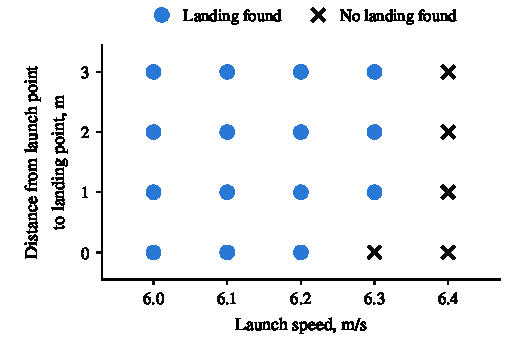
\includegraphics[width=3.4in]{figures/hopring.pdf}
\caption{A 4-s hop of a gimbaled rigid body launched straight up: landing distances at which a nonconvex solver did and did
not find a trajectory.}\label{fig:ring}
\end{figure}

\section{What Remains Possible}\label{sec:possible}
Theorem~\ref{thm:A} excludes a program that is sound and complete. Each weaker goal is attainable.

\emph{A fixed attitude history.} If the body-axis history $b(t)$ is chosen in advance, what remains is a 3-DOF problem with a
pointing cone about a time-varying axis, and the argument of Ref.~\cite{acikmese2013} applies to it: by Aumann's theorem the
relaxed and original problems have the same feasible data. The nonconvexity is entirely in the choice of the attitude.
Successive convexification can be read as a search over that choice.

\emph{Soundness without completeness.} A convex program may be feasible only at landable data, and return a landing there,
without being feasible at all of them. Theorem~\ref{thm:A} does not constrain such a program, since its projection is a
convex subset of $\F$ and need not equal it. One exists for the gimbaled rigid body of Sec.~\ref{sec:tvc}. The center of
percussion $y=r+\varepsilon b$ obeys $\ddot y=(T_a/m-\varepsilon\norm{\dot b}^2)\,b-g_0\ez$, where $T_a$ is the axial
thrust, so the body axis is the direction of $\ddot y+g_0\ez$, and the attitude, the gimbal angle, and the throttle are
algebraic functions of $y$ and its first four derivatives. Planning $y$ as a spline makes the dynamics and the boundary
conditions linear, and the actuator limits can be imposed as second-order cone restrictions on the control points of the
spline that imply the true limits at every instant. The result is one second-order cone program, each feasible point of
which is a trajectory of the rigid body within its limits \cite{repo}. On the cases we studied it gives up about 0.1\% of
fuel and at most 0.4~s of minimum flight time. In the experiment of Fig.~\ref{fig:ring} it is infeasible in all 20
cells: it never reports a landing that does not exist, and at this final time it also gives up the 15 that do.

\emph{Completeness without soundness.} A relaxation such as 3-DOF LCvx with added attitude constraints is complete, and it
is useful as a bound and as an initial guess. Its solutions must be checked, because it is feasible on the whole convex hull
of the landing set.

It follows that the conclusion sometimes drawn from the difficulty of 6-DOF guidance, that the attitude-coupled problem
requires an iterative method, is not what the theorem says. What it says is that a single convex program must give up
either some landings or the guarantee that its answer is one.

\section{Conclusion}
Lossless convexification cannot be extended to powered descent with a rate-limited attitude within the class of programs
to which it belongs. The reason is geometric and independent of any particular relaxation: an exact convex program would
make the set of landable initial states convex, and a dive to one side followed by a brake, together with its mirror image,
shows that the set is not convex, at every final time, under altitude and glide-slope constraints, with depleting mass, for
upright touchdown, and for 6-DOF attitude kinematics. These statements are machine-checked. The proved gap is small for
descents that begin in the air, and for a vehicle steered only by its gimbal the result is proved under simplifying
assumptions at four final times and is otherwise numerical. Open problems are a certificate that accounts for a gimbal-rate
limit and depleting mass, and a bound on the gap that is large enough to matter for short hops, where the numerical
evidence shows a hole in the set of reachable landing points.

\section*{Acknowledgments}
% AIAA policy (Ethical Standards, Sec. 3) requires a description of AI use here and a disclosure at submission.
% The first two sentences below are a factual description of how this work was produced. Complete the rest truthfully.
An artificial-intelligence system (Claude, Anthropic) was used extensively in this work. It derived and wrote the proofs,
wrote the Lean formalization and the numerical software, ran the numerical experiments, and drafted the text and figures of
this manuscript. [State here what the Contributing Student Authors did themselves, for example: posed the question, directed
the investigation, and checked the derivations, the formal statements, and the results.] The independent check described in
Sec.~\ref{sec:lean} was carried out by [name of the reviewer, with permission], who found the missing condition in (S1).
[State any other contributors and sponsors.] The authors are responsible for the content of the paper.

\begin{thebibliography}{99}
\bibitem{acikmese2007} A\c{c}{\i}kme\c{s}e, B., and Ploen, S. R., ``Convex Programming Approach to Powered Descent Guidance for Mars
Landing,'' \emph{Journal of Guidance, Control, and Dynamics}, Vol.~30, No.~5, 2007, pp.~1353--1366. \url{https://doi.org/10.2514/1.27553}.
\bibitem{blackmore2010} Blackmore, L., A\c{c}{\i}kme\c{s}e, B., and Scharf, D. P., ``Minimum-Landing-Error Powered-Descent Guidance for
Mars Landing Using Convex Optimization,'' \emph{Journal of Guidance, Control, and Dynamics}, Vol.~33, No.~4, 2010, pp.~1161--1171.
\url{https://doi.org/10.2514/1.47202}.
\bibitem{acikmese2011} A\c{c}{\i}kme\c{s}e, B., and Blackmore, L., ``Lossless Convexification of a Class of Optimal Control Problems
with Non-Convex Control Constraints,'' \emph{Automatica}, Vol.~47, No.~2, 2011, pp.~341--347. \url{https://doi.org/10.1016/j.automatica.2010.10.037}.
\bibitem{acikmese2013} A\c{c}{\i}kme\c{s}e, B., Carson, J. M., and Blackmore, L., ``Lossless Convexification of Nonconvex Control Bound
and Pointing Constraints of the Soft Landing Optimal Control Problem,'' \emph{IEEE Transactions on Control Systems Technology},
Vol.~21, No.~6, 2013, pp.~2104--2113. \url{https://doi.org/10.1109/TCST.2012.2237346}.
\bibitem{harris2014} Harris, M. W., and A\c{c}{\i}kme\c{s}e, B., ``Lossless Convexification of Non-Convex Optimal Control Problems for
State Constrained Linear Systems,'' \emph{Automatica}, Vol.~50, No.~9, 2014, pp.~2304--2311. \url{https://doi.org/10.1016/j.automatica.2014.06.008}.
\bibitem{malyuta2022} Malyuta, D., Reynolds, T. P., Szmuk, M., Lew, T., Bonalli, R., Pavone, M., and A\c{c}{\i}kme\c{s}e, B., ``Convex
Optimization for Trajectory Generation: A Tutorial on Generating Dynamically Feasible Trajectories Reliably and Efficiently,''
\emph{IEEE Control Systems Magazine}, Vol.~42, No.~5, 2022, pp.~40--113. \url{https://doi.org/10.1109/MCS.2022.3187542}.
\bibitem{mao2016} Mao, Y., Szmuk, M., and A\c{c}{\i}kme\c{s}e, B., ``Successive Convexification of Non-Convex Optimal Control Problems
and Its Convergence Properties,'' \emph{2016 IEEE 55th Conference on Decision and Control}, IEEE, 2016, pp.~3636--3641.
\url{https://doi.org/10.1109/CDC.2016.7798816}.
\bibitem{szmuk2018} Szmuk, M., and A\c{c}{\i}kme\c{s}e, B., ``Successive Convexification for 6-DoF Mars Rocket Powered Landing with
Free-Final-Time,'' AIAA Paper 2018-0617, Jan. 2018. \url{https://doi.org/10.2514/6.2018-0617}.
\bibitem{szmuk2020} Szmuk, M., Reynolds, T. P., and A\c{c}{\i}kme\c{s}e, B., ``Successive Convexification for Real-Time
Six-Degree-of-Freedom Powered Descent Guidance with State-Triggered Constraints,'' \emph{Journal of Guidance, Control, and
Dynamics}, Vol.~43, No.~8, 2020, pp.~1399--1413. \url{https://doi.org/10.2514/1.G004549}.
\bibitem{lean4} de Moura, L., and Ullrich, S., ``The Lean 4 Theorem Prover and Programming Language,'' \emph{Automated Deduction --
CADE 28}, Lecture Notes in Computer Science, Vol.~12699, Springer, Cham, 2021, pp.~625--635. \url{https://doi.org/10.1007/978-3-030-79876-5_37}.
\bibitem{mathlib} The mathlib Community, ``The Lean Mathematical Library,'' \emph{Proceedings of the 9th ACM SIGPLAN International
Conference on Certified Programs and Proofs}, ACM, New York, 2020, pp.~367--381. \url{https://doi.org/10.1145/3372885.3373824}.
\bibitem{repo} Propulsive Landers at Georgia Tech, ``lossless-navigation-paper: Lean Proofs, Certificates, and Guidance Software for
Powered Descent,'' software and data repository, 2026. \url{https://github.com/Propulsive-Landers-GT/lossless-navigation-paper}.
\bibitem{lasserre2008} Lasserre, J. B., Henrion, D., Prieur, C., and Tr\'elat, E., ``Nonlinear Optimal Control via Occupation Measures
and LMI-Relaxations,'' \emph{SIAM Journal on Control and Optimization}, Vol.~47, No.~4, 2008, pp.~1643--1666.
\url{https://doi.org/10.1137/070685051}.
\bibitem{aumann1965} Aumann, R. J., ``Integrals of Set-Valued Functions,'' \emph{Journal of Mathematical Analysis and Applications},
Vol.~12, No.~1, 1965, pp.~1--12. \url{https://doi.org/10.1016/0022-247X(65)90049-1}.
\bibitem{ipopt} W\"achter, A., and Biegler, L. T., ``On the Implementation of an Interior-Point Filter Line-Search Algorithm for
Large-Scale Nonlinear Programming,'' \emph{Mathematical Programming}, Vol.~106, No.~1, 2006, pp.~25--57. \url{https://doi.org/10.1007/s10107-004-0559-y}.
\end{thebibliography}
\end{document}
